\documentclass[xcolor=table]{beamer}
\input{style}
\input{macros}

\author{Malte Schmitz}
\title{LaTeX}
\date{MetaNook 2016}

\begin{document}

%!TEX root = tikz.tex

\begin{frame}
  \begin{center}
    \vskip1cm
    {\bfseries\color{maincolor}{\Huge\rmfamily
    Zeichnen in \LaTeX{} mit}}
    \par\vskip5mm
    {\bfseries\color{maincolor}\fontsize{72pt}{72pt}\selectfont\rmfamily\TikZ}
    \par\vskip12mm
    \large Malte Schmitz
  \end{center}
\end{frame}
%!TEX root = tikz.tex

\begin{frame}{Ziele dieser Vorlesung}
  \begin{itemize}
    \item \TikZ\ kennen und lieben lernen.
    \item Pfade mit \TikZ\ zeichnen können.
    \item Das Konzept von Knoten und deren Positionierung verstehen.
    \item Animationen mit \TikZ\ und Beamer kennen lernen.
  \end{itemize}
\end{frame}

\begin{frame}{Gliederung}
  \tableofcontents
\end{frame}

\begin{frame}{Website}
  \vskip-4ex\hfill\parbox{6cm}{\centering
    \includegraphics[width=6cm]{qrcode}\\[1ex]
    \href{http://www.mlte.de/latex}{\huge\texttt{mlte.de/latex}}}
  \begin{itemize}
    \item Diese Präsentation.
    \item Das Skript zum Vortrag.
    \item Beispieldokumente, Links zu weiteren Quellen.
    \item Skripte, Folien und Videos aus den Vorjahren.
  \end{itemize}
\end{frame}


\section{Einführung}

\begin{frame}{Was ist \TikZ?}
  \begin{itemize}
    \item \TikZ\ ist kein Zeichenprogramm,\\
      dient aber zum Zeichnen von Grafiken mit \LaTeX.
    \item \TikZ\ ist ein Makropaket für \TeX\ bzw. \LaTeX.
    \item \TikZ\ verfügt über eine sehr ausführliche und gute Anleitung.
  \end{itemize}
\end{frame}

\subsection{Pfade}

\begin{frame}{Pfade}
  \begin{itemize}
    \item Ein Pfad ist eine Folge von Koordinaten.
      \begin{itemize}
        \item Links unten ist der Ursprung \lstinline-(0,0)-,
        \item die erste Koordinate geht nach rechts und
        \item die zweite Koordinate geht nach oben.
      \end{itemize}
    \item Eine Linie wird mit \lstinline|--| gezeichnet.
    \item Relative Koordinaten beginnen mit \lstinline-++-.
  \end{itemize}
\end{frame}

\begin{Frame}{Unser erstes Ziel}
  \centering
  \begin{tikzpicture}[scale=4]
    % Gitter im Hintergrund
    \draw[step=.5cm,gray,very thin] (0,0)
      grid (1.4,1.4);
    % Kreisbogen
    \draw (1,0) arc (0:90:1cm);
    % Koordinatenachsen
    \draw[->] (0,0) -- (1.5,0) node[right] {$x$};
    \draw[->] (0,0) -- (0,1.5) node[above] {$y$};
    \draw (1,1pt) -- (1,-1pt) node[below] {$1$};
    \draw (1pt,1) -- (-1pt,1) node[left] {$1$};
    % Winkel
    \filldraw[fill=green!20,draw=green!50!black]
      (0,0) -- (3mm,0pt) arc (0:30:3mm);
    \draw (15:2mm) node[green!50!black] {$\alpha$};
    % Sinus und Kosinus
    \draw[very thick,red]
      (30:1cm) -- node[left]
        {$\sin \alpha$} (30:1cm |- 0,0);
    \draw[very thick,blue]
      (0,0) -- node[below]
        {$\cos \alpha$} (30:1cm |- 0,0);
    % Schnittpunktberechnung und Tangens
    \path [name path=upward line]
      (1,0) -- (1,1);
    \path [name path=sloped line]
      (0,0) -- (30:1.5cm);
    \draw [name intersections=
      {of=upward line and sloped line, by=tan}]
      [very thick,orange] (1,0) -- node [right]
      {$\displaystyle \tan \alpha \color{black}=
        \frac{{\color{red}\sin \alpha}}
          {\color{blue}\cos \alpha}$} (tan);
    \draw (0,0) -- (tan);
  \end{tikzpicture}
\end{Frame}

\livecoding{Einführung}

\section{Graphen}

\subsection{Knoten}

\begin{frame}{Wofür Knoten?}
  \begin{itemize}
    \item \alert{Wir können jetzt alles zeichnen.}
    \item Viele Zeichnungen basieren auf Graphen,
      bestehen also aus Knoten und Kanten.
      \begin{itemize}
        \item Automaten
        \item UML-Diagramme
        \item Stoffwechselwege
        \item Ablaufdiagramme
      \end{itemize}
    \item Solche Diagramme mit Kreisen und Linien zu zeichnen erzeugt
      \alert{unübersichtlichen und schlecht wartbaren} \LaTeX-Code.
  \end{itemize}
\end{frame}

\begin{frame}{Ziel Knoten}
  \centering
  \begin{tikzpicture}
    [io/.style={trapezium, trapezium left angle=70, trapezium right angle=110, fill=magenta!10, draw=magenta},
    op/.style={rectangle, fill=orange!10, draw=orange},
    cn/.style={diamond, aspect=2, inner sep=2pt, fill=red!10, draw=red},
    node distance=5mm, thick]
    \node[io] (in) {Eingabe $a,b$};
    \node[op, below=of in] (div) {$r=a \mod b$};
    \node[op, below=of div] (set) {$a=b,\ b=r$};
    \node[cn, below=of set] (cond) {$b=0?$};
    \node[io, below=of cond] (out) {Ausgabe $a$};
    %
    \path[->]
      (in) edge (div)
      (div) edge (set)
      (set) edge (cond)
      (cond) edge node[right] {Ja} (out);
    \draw[->] (cond) -- node[below] {Nein} ++(1.5,0) |- (div);
  \end{tikzpicture}
\end{frame}

\livecoding{Knoten}

\subsection{Automaten}

\begin{frame}{Ziel Automaten}
  \centering
  \begin{tikzpicture}[auto, thick]
    \node[initial,state] (q0) {$q_0$};
    \node[state, right=of q0] (q1) {$q_1$};
    \node[state, accepting, right=of q1] (q2) {$q_2$};
    \path
      (q0) edge[->] node {0} (q1)
      (q1) edge[->, loop above] node {0} ()
      (q1) edge[->, bend left] node {1} (q2)
      (q2) edge[->, bend left] node {0} (q1);
  \end{tikzpicture}
\end{frame}

\livecoding{Automaten}

\subsection{Bäume}

\begin{frame}{Ziel Bäume}
  \tikzset{
    every node/.style={
      draw,
      circle,
      inner sep=0pt,
      minimum width=15pt
    },
    thick
  }

  \centering
  \begin{tikzpicture}
    \node {a}
      child { node {b}
        child { node {d} }
        child { node {e} }
      }
      child { node {c}
        child { node {f} }
        child { node {g} }
      };
  \end{tikzpicture}
\end{frame}

\livecoding{Bäume}

\subsection{Funktionsplots}

\begin{frame}{Ziel Funktionsplots}
  \centering
  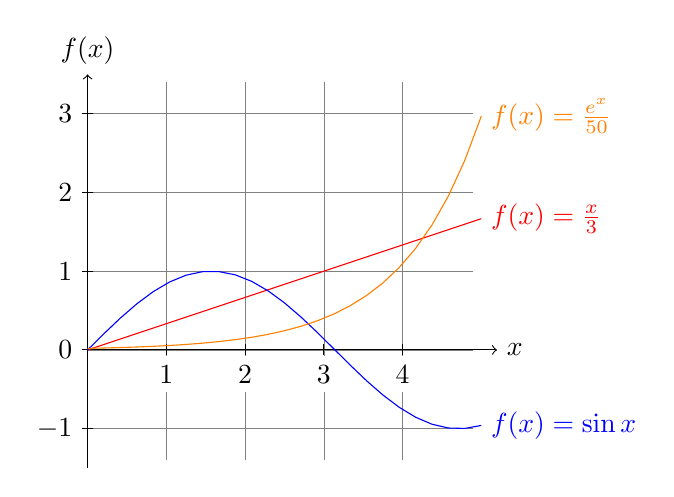
\begin{tikzpicture}[domain=0:5]
    \draw[very thin,gray] (0,-1.4) grid (4.9,3.4);
    \draw[->] (0,0) -- (5.2,0) node[right] {$x$};
    \draw[->] (0,-1.5) -- (0,3.5) node[above] {$f(x)$};
    %
    \foreach \x in {1,...,4}
      \draw[xshift=\x cm] (0,2pt) -- (0,-2pt) node[below,fill=white] {$\x$};
    \foreach \y in {-1,...,3}
      \draw[yshift=\y cm] (2pt,0) -- (-2pt,0) node[left,fill=white] {$\y$};
    %
    \draw[red]    plot (\x,\x/3)         node[right] {$f(x) = \frac{x}{3}$};
    \draw[blue]   plot (\x,{sin(\x r)})  node[right] {$f(x) = \sin x$};
    \draw[orange] plot (\x,{exp(\x)/50}) node[right] {$f(x) = \frac{e^x}{50}$};
  \end{tikzpicture}
\end{frame}

\livecoding{Funktionsplots}

\section{Beamer}

%!TEX root = tikz.tex

\begin{frame}{Was ist \beamer?}
  \begin{itemize}
    \item \alert{Dokumentenklasse für \LaTeX} für die Erzeugung von Präsentationen.
      \only<article>{\newline(Diese Präsentation und das Skript wurden mit \beamer\ erzeugt.)}
    \item Keine eigene und \alert{keine graphische Anwendung}.
    \item \strut\beamer\ ist in vielen \TeX-Distributionen enthalten.\newline
      (\alert{Es kann direkt losgehen}.)
  \end{itemize}
\end{frame}

\begin{frame}{Workflow}
  \lstset{language={}}
  \begin{enumerate}
    \item Normales \LaTeX-Dokument erzeugen.\\
      Dabei einige spezielle \beamer-Kommandos verwenden.
    \item \LaTeX-Dokument mit \lstinline-pdflatex- kompilieren.
    \item Ergebnis überprüfen und \LaTeX-Dokument anpassen.
  \end{enumerate}
\end{frame}

\begin{frame}[fragile]{Folien}
  \begin{itemize}
    \item Ein \beamer-Dokument besteht aus mehreren Frames.
    \item Jeder Frame kann aus mehreren Slides bestehen.
    \item Die Umgebung \lstinline-frame- verarbeitet
      bis zu zwei Parameter in gescheiften Klammern \lstinline-{}-
    \item Der erste Parameter ist der Titel.
    \item Der zweite Parameter ist der Untertitel.
    \item Innerhalb der Umgebung \lstinline|frame| wird normaler \LaTeX-Code
      verwendet.
  \end{itemize}
\end{frame}



\livecoding{Beamer}

% REGIE: Theme-Matrix zeigen

\subsection{Overlays}

\subsection{Overlays mit \TikZ}

\subsection{Artikelfassung}

\input{beamer-article}

%!TEX root = tikz.tex

\begin{frame}{Zusammenfassung}
  \begin{enumerate}
    \item \TikZ-Zeichnungen bestehen aus \alert{Pfaden}, die über \alert{Koordinaten} definiert werden.
    \item Fast alle scheamtischen Zeichnungen sind ein \alert{Graph}, bestehen also aus \alert{Knoten} und \alert{Kanten} und
      werden auch als solche in \TikZ\ gezeichnet.
    \item Mit der Dokumentenklasse \lstinline-beamer- können \alert{sehr
      leicht Präsentationen erstellt} werden, wenn man mit \LaTeX\ etwas geübt ist.
    \item \alert{Overlay-Spezifikationen} werden in spitzen
      Klammern \lstinline-<- und \lstinline->- angegeben. Diese beeinflussen, in welchem
      \alert{Schritt der Animation} das Kommando ausgeführt wird.
    \item Bei Problemen und Fragen \alert{lies die Anleitung!}
  \end{enumerate}
\end{frame}

\begin{frame}{Zum Weiterlesen}
  \begin{mybib}
    \bibitem{Tantau4}
      Till Tantau.
      \newblock \emph{The \TikZ\ and \textsc{pgf} Packages},
      \newblock Manual for version 2.10,
      \newblock \alt<presentation>{\href{http://mirrors.ctan.org/graphics/pgf/base/doc/generic/pgf/pgfmanual.pdf}{\texttt{pgfmanual.pdf}}}{\url{http://mirrors.ctan.org/graphics/pgf/base/doc/generic/pgf/pgfmanual.pdf}}, Oktober 2010.

    \bibitem{Texample}
      Kjell Magne Fauske und Stefan Kottwitz.
      \newblock \emph{\TeX ample.net},
      \newblock ample resources for TeX users,
      \newblock \alt<presentation>{\href{http://www.texample.net/tikz/examples/}{\texttt{texample.net}}}{\url{http://www.texample.net/tikz/examples/}}.
  \end{mybib}
\end{frame}

\begin{frame}{Zum Weiterlesen (Beamer)}
  \begin{mybib}
    \bibitem{Tantau}
      Till Tantau, Joseph Wright und Vedran Mileti\'c.
      \newblock The \textsc{beamer} \textit{class}, User Guide.
      \newblock \alt<presentation>{\href{http://mirrors.ctan.org/macros/latex/contrib/beamer/doc/beameruserguide.pdf}{\texttt{beameruserguide.pdf}}}{\url{http://mirrors.ctan.org/macros/latex/contrib/beamer/doc/beameruserguide.pdf}}, Oktober 2013.

    \bibitem{Tantau}
      Till Tantau.
      \newblock \emph{Beamer: Strahlende Vorträge mit \LaTeX},
      \newblock Präsentieren und Dokumentieren -- Tools.
      \newblock Vorlesung vom 31. Oktober 2012.
  \end{mybib}
\end{frame}

\end{document}